\renewcommand{\theequation}{\theenumi}
\begin{enumerate}[label=\arabic*.,ref=\thesubsection.\theenumi]
\numberwithin{equation}{enumi}
\item let probability of head when a single coin is tossed = p
\\
let probability of tails when a single coin is tossed = q
\\
probability of two head when three coins are tossed = P(X=2)
\begin{align}
p &= \frac{1}{2}
\\
q &= \frac{1}{2}
\\
P(X=2) &= ^nC_k \times \left(p\right)^n \left(q\right)^{1-n}\left(\text{binomial theoram}\right)
\\
P(X=2) &= ^3C_2 \times \left(\frac{1}{2}\right)^2 \left(\frac{1}{2}\right)^1
\\
&= \frac{3}{8}
\end{align}
codes for the above equation can be get from here
\begin{lstlisting}
codes/prob/prob4.py
\end{lstlisting}
\begin{figure}[!ht]
	\centering
	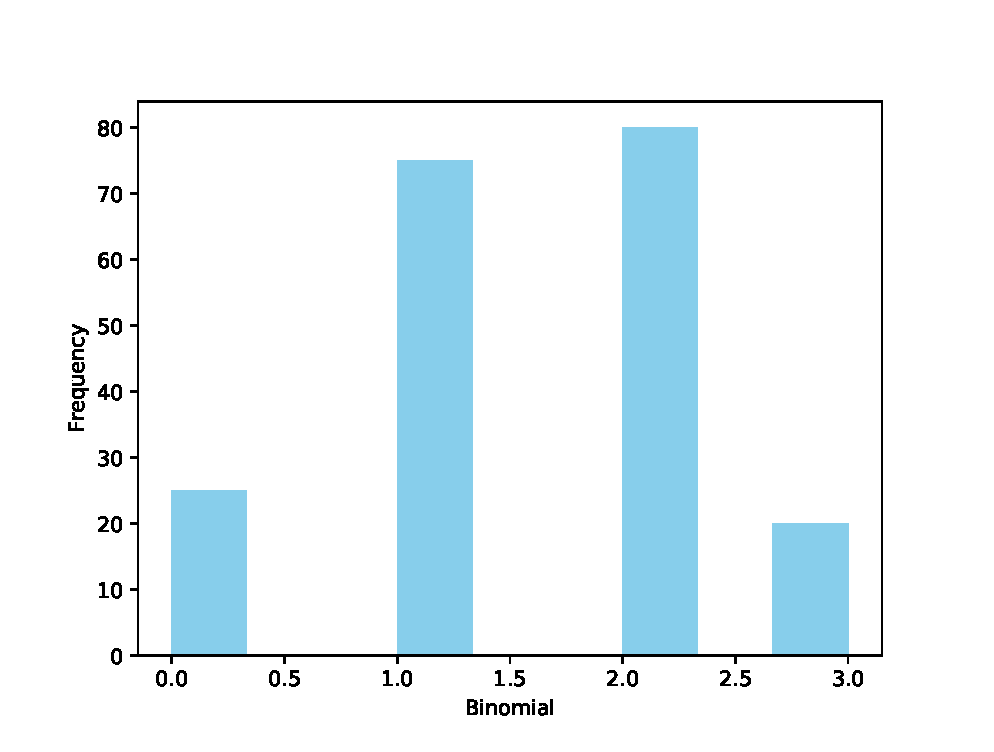
\includegraphics[width=\columnwidth]{./figures/prob/prob4.eps}
	\caption{binomial distribution of toss of three coins }
	\label{fig:bt2}
	\begin{lstlisting}
	figs/prob/prob4.py
	\end{lstlisting}
\end{figure}
\end{enumerate}